
%%%%%%%%%%%%%%%%%%%%%%%%%%%%%%%%%%%%
%{Background and Literature Review}%
%%%%%%%%%%%%%%%%%%%%%%%%%%%%%%%%%%%%

%{summary for all the literature review}

%{ classification of motion models }
Motion planning for autonomous vehicles has been studied extensively to provide optimal and collision-free trajectories\cite{motion_planning}. Most algorithms assume known trajectories of all surrounding agents, while in fact we have very limited information about  vehicles around us. Predicting surrounding vehicles' movements enables more active and more practical traffic studies. In the following section, based on the method employed, motion prediction models are classified into three main categories, namely physics-based models, driver behavior models and interactive models.

%Without in-traffic direct communications or high-level traffic commands, existing assumption is not realistic. 

\subsection{Physics-Based Models}
\label{Literature:Physics-Based}
Physics-based motion predictions use dynamic or kinematic models governed by simple physics laws as surveyed by Lef{\`e}vre et al. in \cite{survey_motion_prediction}.  These physics-based models predict the possible motion of the surrounding agents adopt  linear-velocity models for their efficiency, friendiness in use, and good accuracy in short-term predictions\cite{physics_real_time, physics_velocity_obstacle}. However, they do not account for uncertainties in real traffic with other human drivers. Zhan et al. use  probability models of yielding/passing actions at a crossroad\cite{non-conservative}. Other prediction models such as the work of Ruf et al. \cite{sparc} use a cost map with probabilistic values on each path to optimize the global planner of vehicle movements. Although physics-based models are easier and cheaper to be applied, they suffer from poor long-term predictions, therefore have little interactions between the ego vehicle and other agents.

% \begin{figure}[htbp]
% \begin{center}
% 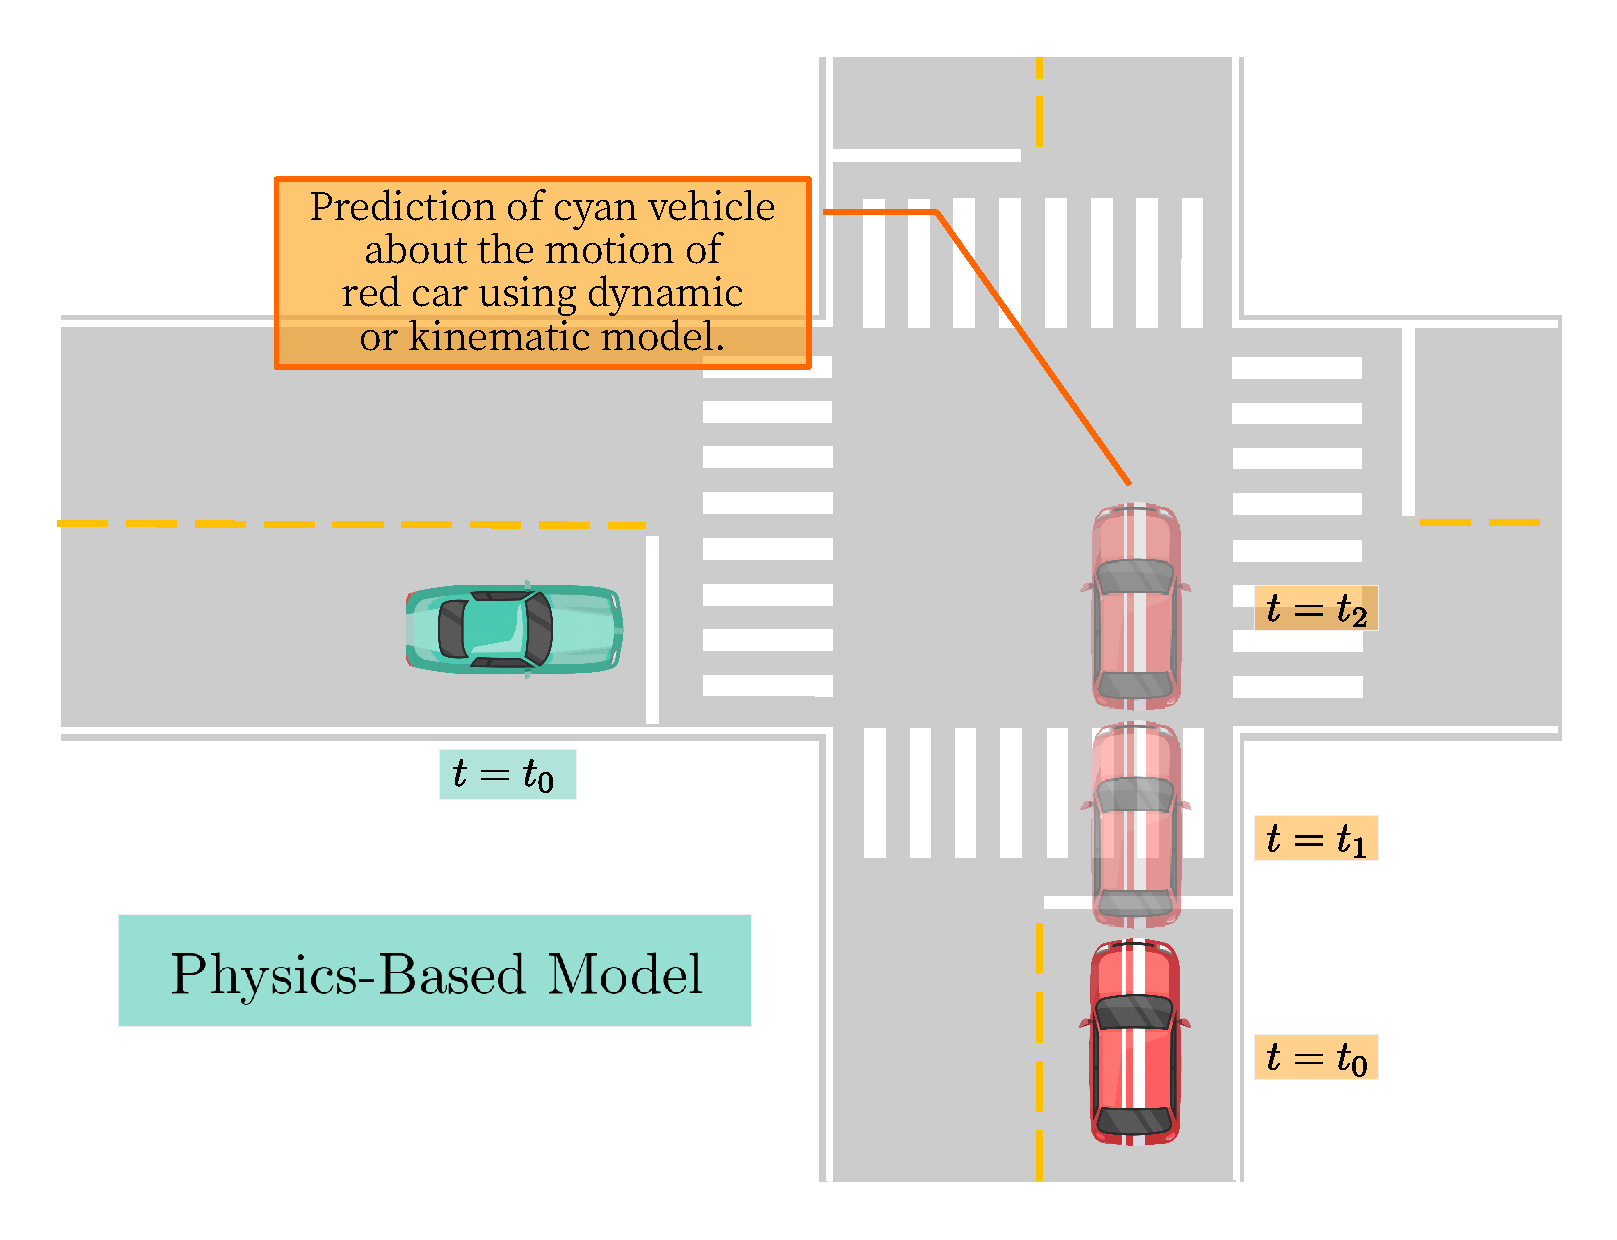
\includegraphics[scale=0.3]{intersection_physics.pdf}
% \end{center}
% \caption{Physics-Based Model.}
% \label{physics-based} 
% \end{figure}


\subsection{Driver Behavior Models}
\label{Literature:Driver Behavior}
Motion predictions with driver behavior models on gas pedals/braes/steers along a path are the intent recognition processes based on the previous and current states of the target agents. Possible behaviors of surrounding agents are listed with a likelihood measure such as Bayesian networks or hidden Markov Model (HMM). Such models can be used, as an example, to estimate the chance of a vehicle violating a stop sign with dynamic Bayesian network (DBN) without extensive trajectory predictions \cite{Lefevre2012}. Dagli et al. \cite{Dagli2003} used the same concept in building vehicle following and lane changing models with sensor data uncertainty as well as uncertainties in human behaviors. Their study is assessed in simulated lane changing experiments where the driver behaviors is recognized 1.5 seconds earlier than the actual lane change. Gindele et al. \cite{Gindele2013} use DBN, combined with the manually formulated models and models learned with random forest tree,  to estimate and predict the driver behaviors of two cars passing an intersection. 

%Online learning is possible in the proposed method where the model would be able to adapt to new environments.

% \begin{figure}[htbp]
% \begin{center}
% 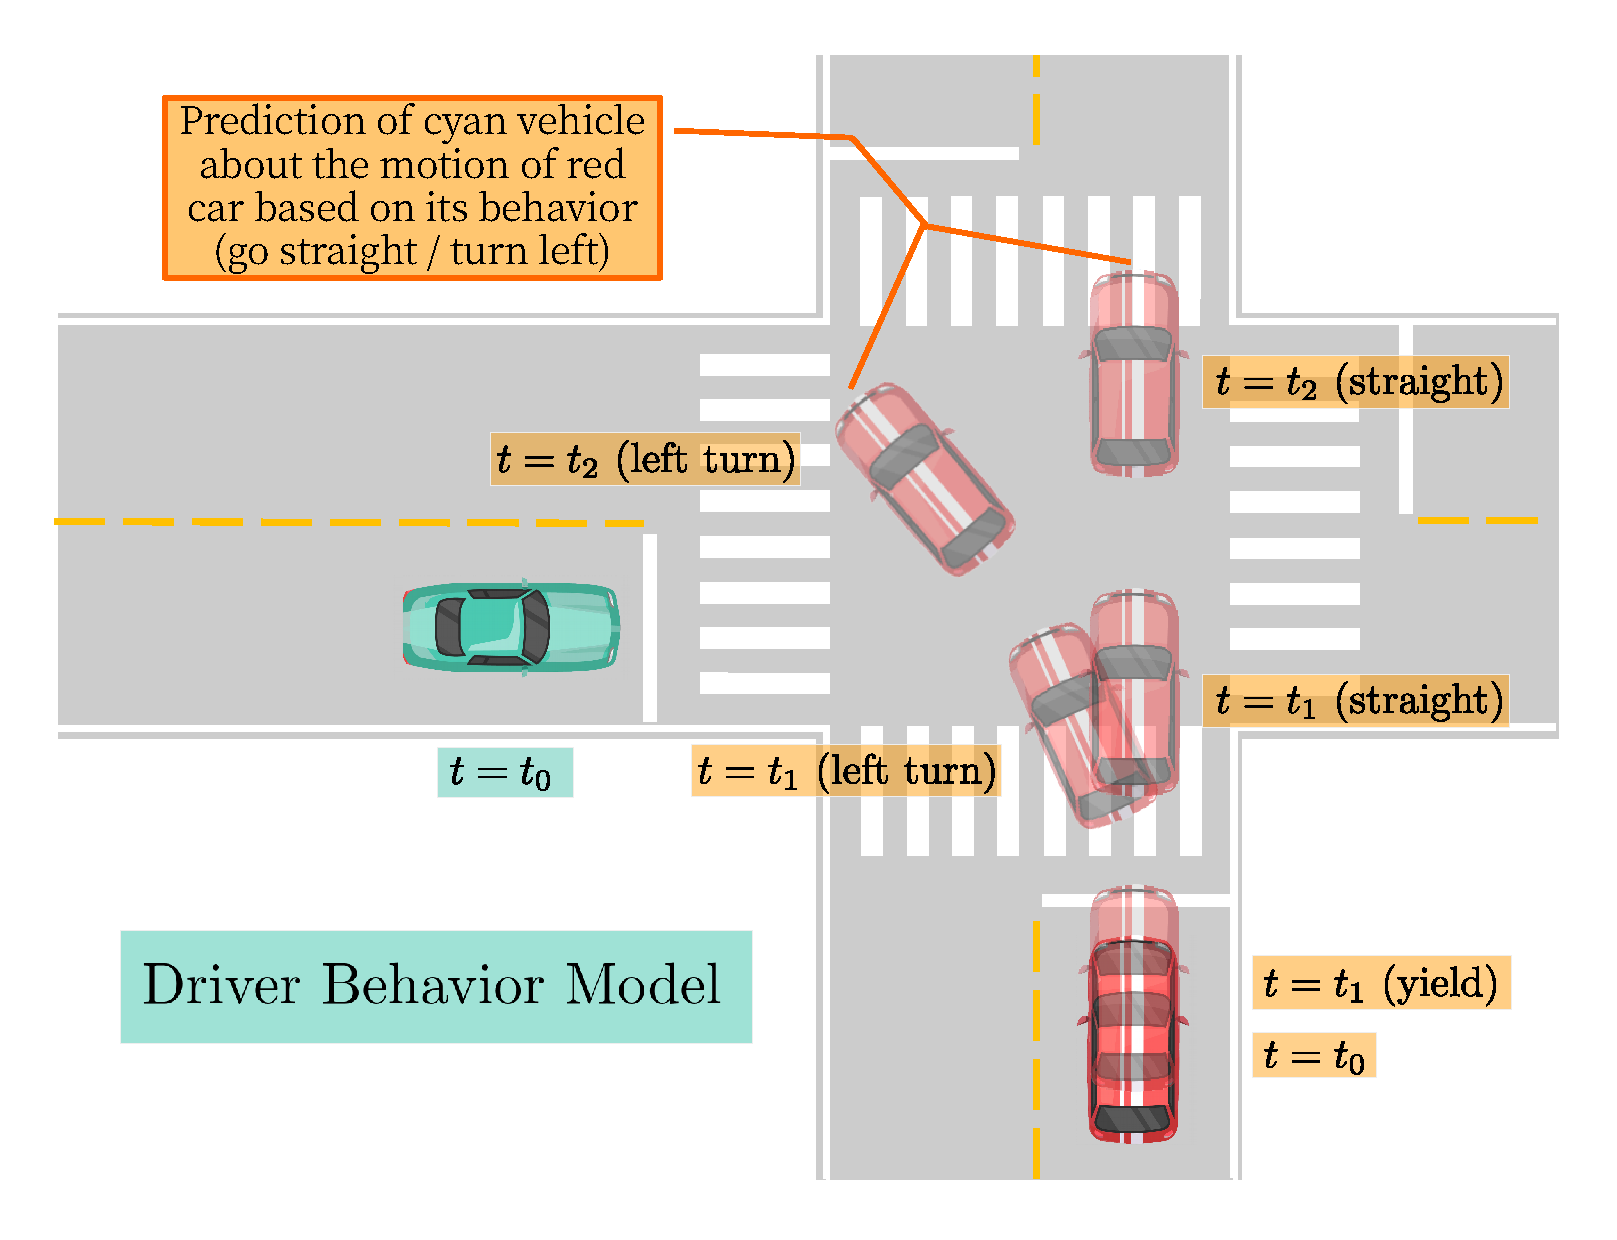
\includegraphics[scale=0.3]{intersection_behavior.pdf}
% \end{center}
% \caption{Driver Behavior Model.}
% \label{driver_behavior} 
% \end{figure}


\subsection{Interactive Models}
\label{Literature:Interactive}
Long-term predictions have been achieved using interactive models with other agents. For example, at a vehicle might decide to pass an intersection because he/she believes that other vehicles are very likely to brake. Probabilistic methods such as partially observable Markov decision process (POMDP) have been used as the core of interactive models to determine the actions of an ego vehicle by predicting the future states of other agents. Foka et al. use FOMDP to navigate in a space with obstacles in \cite{Foka}. Hubmann et al. use POMDP to evaluate the possible maneuvers of other agents and optimize the actions of the ego vehicle in \cite{state_uncertain_environment}. However, POMDP is computationally expensive and therefore unable to be used for  real-time predictions. In addition, vehicle drivers need to predict the trajectories of only nearby vehicles, instead of all, a downsized POMDP application with only nearby vehicles is needed.

% \begin{figure}[htbp]
% \begin{center}
% 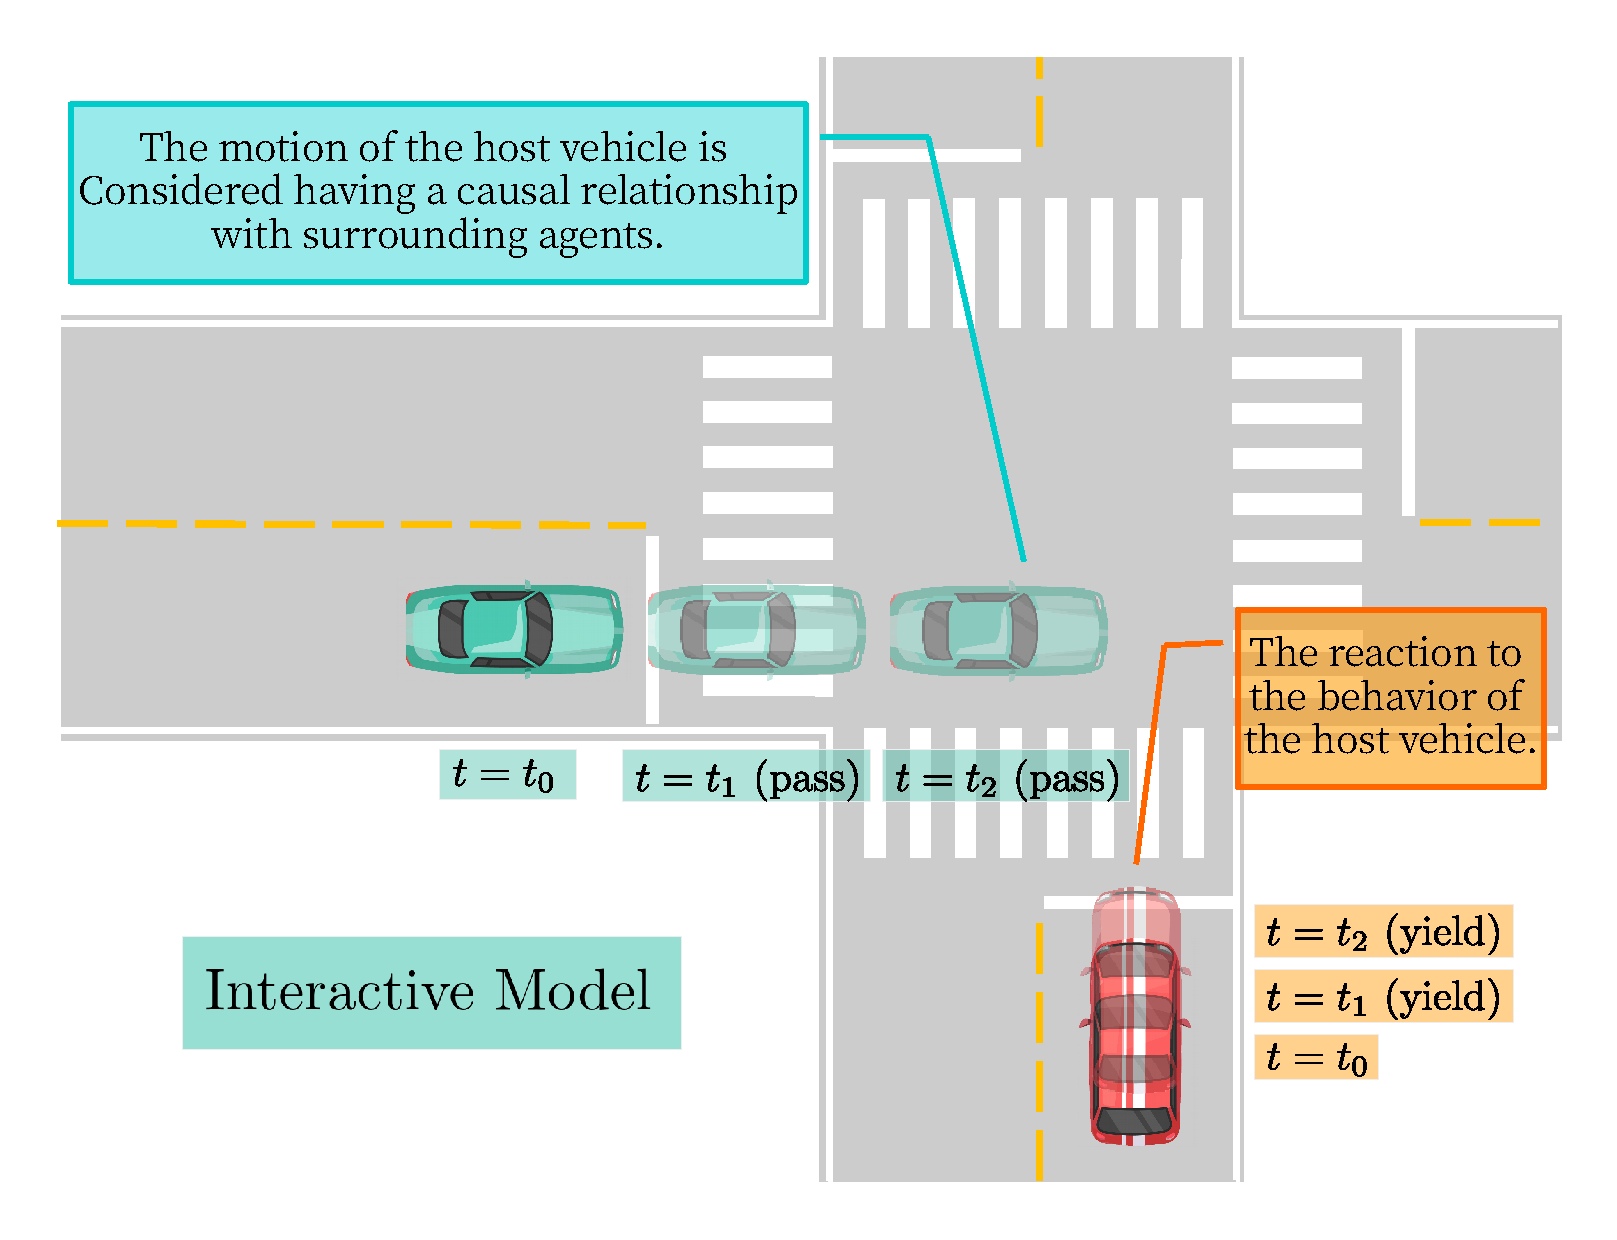
\includegraphics[scale=0.3]{intersection_interactive.pdf}
% \end{center}
% \caption{Interactive Model.}
% \label{interactive} 
% \end{figure}



\subsection{Explicit Driver Behavior Models}

Behavior models provide driver intent for predictions in urban intersection that form the basics for current advance driver assistance systems (ADAS). Liebner et al. use intelligent driver models (IDM) for probability of turning and car-following behaviors in a simple Bayes net in \cite{Liebner2012} with different intention probabilities in arbitrary intersections with general speed profiles. To overcome driver behavior change, the features of different agents, such as speed, distance to the intersection, are extracted by Graf et al. in the process of case-based reasoning (CBR) for site-specific intersections\cite{Graf2014}. CBR relates a case with similar experiences to predict the behavior of the driver. However, the results learned from one intersection still may not directly applicable for other intersections. Drivers with different driving style also affect the prediction accuracy significantly.   

\subsection{Summary}
Despite the explicit formulation and general applicability, physics-based models can not account for states changes of the subject, which results in the poor long-term prediction. Interactive models with joint behaviors of surrounding agents could achieve better long-term predictions, with the sacrifice of  computational cost and unable to handle large state spaces. Driver behavior models, on the other hand, have better long-term estimations than physics-based models \ref{Literature:Physics-Based} and better computational efficiency than interactive models \ref{Literature:Interactive} trained models are, however, only applicable to environments where the training data are extracted. More general and explicit driver behavior models at various traffic scenarios are needed to smoothly blend into urban traffic with mixed fleet. Each driver needs to understand the behaviors and intentions of other road users so that they can and react accordingly. 

Autonomous vehicles nowadays do have the ability to resolve some potential threats, actively maneuver vehicles to avoid obstacles; however, they usually do so with no regard of what the maneuvers are perceived by human drivers. While technology can observe what's going on based on captured evidences, intentions are more subtle than behaviors. Human drivers can pass the interactions by predicting the intention of the other agents : accelerate to pass or decelerate to yield. Since humans don't perceive the world numerically, researchers have suggested that instead of calculating the distance and the speed directly to learn the time to hit an object, human drivers adopt a more cognitive and abstract methods \cite{cog}.

In this work the driver behavior models is chosen for its better long-term prediction and computational efficiency compared to the other two models.  Hence, in the following chapters, an explicit driver behavior models will be developed to account for driver behaviors at various traffic scenarios.

